\subsection{MAC grid}

When storing quantites on a grid, it is common to store the values at the center of each cell. This approach can be tempting to use since it makes implementations clean and simple. However, there are different ways to store the quantites and it values do not necessary have to be stored at the center of the cell. An example of this is the MAC grid introduced by Harlow and Welch in 1965.

\begin{figure}[ht!]
\centering
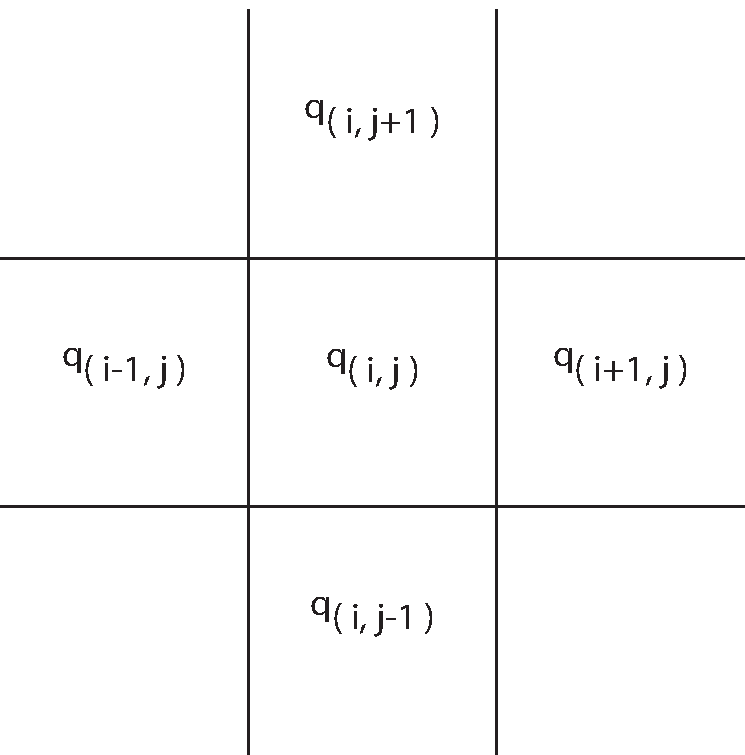
\includegraphics[width=40mm]{img/mac.pdf}
\caption{A grid with quantity $q$ stored at the center of the cells.}
\label{regulargrid}
\end{figure}

Before we talk about the difference of a regular grid and a MAC grid, let us revisit derivate approximations in a grid with fixed amount of samples. Figure 2 shows a simple 2D-dimensional grid with the quanity $q_{i,j}$ stored at the center of each cell. To estimate the derivate of q in the x-direction, we can either use first order forward difference 

\begin{equation}
(\frac{\partial q}{\partial x})_{i,j} \approx \frac{q_{i+i,j} - q_{i,j}}{\Delta x}
\end{equation}

accurate to $O(\Delta x)$ or use first order central difference

\begin{equation}
(\frac{\partial q}{\partial x})_{i,j} \approx \frac{q_{i+i,j} - q_{i-1,j}}{2\Delta x}
\label{centraldifference}
\end{equation}

that has accuracy proportional to $O(\Delta x^{2})$. Even though central difference is more accurate, we can make it even more accurate without having to use complicated approximations. To solve the Navier-Stokes equations we are later on going to need to approximate partial derivates of both the velocity field $\vec{u}$ and the pressure field $\rho$. As we will see in later sections of this report, the partial derivate of the pressure field $\frac{\partial \rho}{\partial x}$ is going to be evaluated to update the velocity field $\vec{u}$. In a similar way, we will have to evaluate $\nabla \cdot \vec{u}$ in the linear equations to solve for pressure. This motivates the use of a staggered grid, i.e a grid where different variables are stored at different locations in the grid.

\begin{figure}[ht!]
\centering
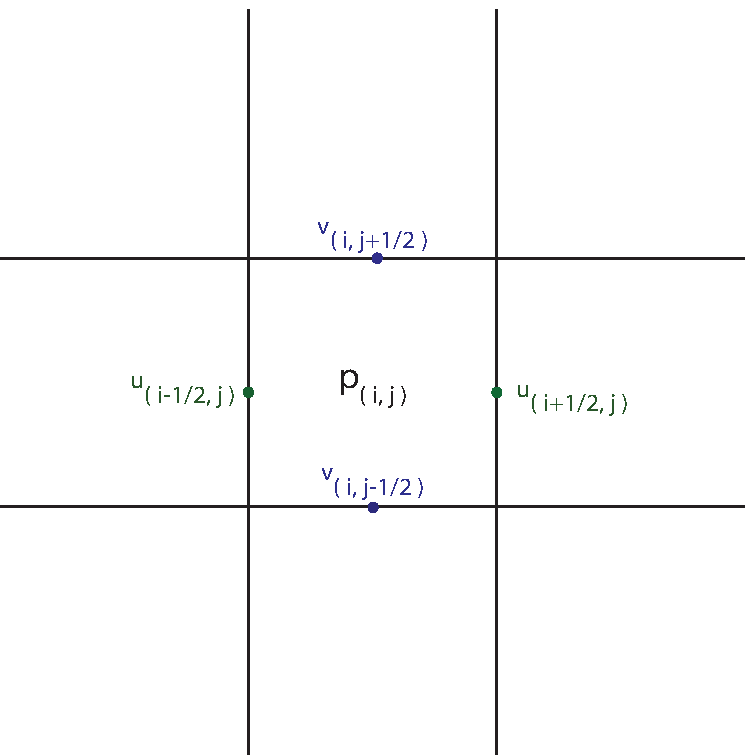
\includegraphics[width=60mm]{img/mac2.pdf}
\caption{A MAC grid with pressure $p$ stored at the center of the cell and velocties $u$ and $v$ stored on the edges.}
\label{macgrid}
\end{figure}

In Figure \ref{macgrid} we see a two-dimensional MAC grid. A MAC grid, marker-and-cell, stores the pressure $\rho$ at the center of the cell and splits the vector field $\vec{u} = (u,v)$ into a component for each axis and store it on the faces of the cell, i.e in this 2D example it splits $(u,v)$ and stores $u$ on the horizontal faces and $v$ on the vertical ones. At first, this might be confusing but when we evaluate the derivates it should make more sense. To evaluate the divergence of $\vec{u}$ at the center of a cell $(i,j)$, we use central difference on the values stored at the faces

\begin{equation}
\nabla \cdot \vec{u} = \frac{u_{i+1/2,j} - u_{i-1/2,j}}{\Delta x} + 
                       \frac{v_{i,j+1/2} - u_{i,j-1/2}}{\Delta x}
\end{equation}

Compared to Equation \ref{centraldifference}, we only divide by $\Delta x$ instead of $2\Delta x$. In terms of implementation, the staggered grid does not have a larger memory footprint than a regular grid structure. In other ways, we get more accurate derivates without slowing down the performance. To evaluate the derivate of the pressure $\rho$ at a face we perform central difference on neighboring pressure values stored at the center

\begin{equation}
\frac{\partial \rho_{i-1/2,j}}{\partial x} = \frac{\rho_{i,j} - \rho_{i-1,j}}{\Delta x}
\end{equation}

\begin{equation}
\frac{\partial \rho_{i,j-1/2}}{\partial y} = \frac{\rho_{i,j} - \rho_{i,j-1}}{\Delta x}
\end{equation}
